% This is based on the LLNCS.DEM the demonstration file of
% the LaTeX macro package from Springer-Verlag
% for Lecture Notes in Computer Science,
% version 2.4 for LaTeX2e as of 16. April 2010
%
% See http://www.springer.com/computer/lncs/lncs+authors?SGWID=0-40209-0-0-0
% for the full guidelines.
%
\documentclass[runningheads]{llncs}
\usepackage{graphicx}
\usepackage{tikz,pgfplots}
\usepackage[hyphens]{url}
\usepackage[
bookmarks=true,                                      % show bookmarks bar?
%colorlinks=true,                                     % false: boxed links; true: colored links
linkcolor=red,                                       % color of internal links
%linkbordercolor=red,
citecolor=green,                                     % color of links to bibliography
%citebordercolor=green,
%filecolor=magenta,                                   % color of file links
urlcolor=blue,                                       % color of external links
%urlbordercolor=blue,
anchorcolor=black,% Ankertext
%hidelinks=true,
%backref, % Back-Links zu den Kapiteln
pdfborder={0 0 0}
]{hyperref}
\def\UrlBreaks{\do\-\do\_\do\/\do\*\do\~\do\'\do\"\do.}
\usepackage{breakurl}
\newcommand{\MANET}{MANET}
\newcommand{\DOS}{DoS}
\newcommand{\QOS}{QoS}
\newcommand{\VOIP}{VoIP}


\begin{document}

\title{Meeting Data Specific Quality of Service Requirements in Mobile Ad-Hoc Networks with High Network Load}
%Multicast communication in bandwidth restricted Mobile Ad-Hoc Networks
\titlerunning{Data Type Specific QoS In MANETs}  % abbreviated title (for running head)
%                                     also used for the TOC unless
%                                     \toctitle is used
%
\author{Klement Streit \and Peter Hillmann
}
%
\authorrunning{K. Streit, P. Hillmann} % abbreviated author list (for running head)
%
%%%% list of authors for the TOC (use if author list has to be modified)
%\tocauthor{Ivar Ekeland, Roger Temam, Jeffrey Dean, David Grove,
%Craig Chambers, Kim B. Bruce, and Elisa Bertino}
%
\institute{Universit\"at der Bundeswehr M\"unchen, 85579 Neubiberg, Germany\\
\email{\{klement.streit,peter.hillmann\}@unibw.de}}

\maketitle              % typeset the title of the contribution

\begin{abstract}
 In the military sector, radio communication is vital during a mission. The information exchange is provided using a Mobile Ad-Hoc Network. In order to reach specific participants and to transmit data in the awareness of restricted resources, multicast is the common communication technique. Within the network, the armed forces send different data types with appropriate transmission technologies. Hence, the forwarding of video and audio streams over several nodes increases the network load. Different Quality of Service requirements exist for specific data types. Voice has the highest priority and should be delivered in real time. Quality of Service is compromised by overload situations, limited bandwidth, arising bottlenecks or active attacks. These situations can result in higher delay, congestion, insufficient packet delivery and, in the worst case, a Denial of Service. Therefore, the objective of this PhD research is to adapt the transmission of various data types to the current utilization of the Mobile Ad-Hoc Network, to ensure Quality of Service and resilience. For instance, in order to meet the requirements, certain routes within the network that are compromised by limited bandwidth will prioritize transmission of voice over video.

\keywords{MANET, Multicast, QoS, Streaming, Bandwidth Limitation}
\end{abstract}
%
\section{Introduction}\label{sec:Introduction}
%
	The communication via radios between soldiers during a mission is essential and indispensable. The tactical forces have a continuous information exchange within the troop, as well as with other troops. They inform about their current status or exchange mission information. With the Software Defined Radio (SDR) \cite{SDR}, the armed forces have the possibility of transmitting information via the TCP/IP-Stack. Now, the necessary group communication is established via multicast routing, which is an appropriate method to share information between several participants. The soldiers therefore build a Mobile Ad-Hoc Network (\MANET{}). This network structure is well-suited, because a group of soldiers communicating in the field cannot rely on a centralized infrastructure during a mission \cite{military:manet}. The SDR technology also enables the transmission of different data types like video/audio streams, pictures of observations or general file transfer, depending on the  applications running on the radios. With the exchange of different information material, situations can be described more specific.
	
	\section{Problem Description}
	 % A drone could for instance pass a video stream of an observed area to the multicast group or soldiers exchange tactical situation pictures. 
	In the military sector it is particularly important to meet the transmission requirements with Quality of Service (\QOS{}) compared to the civil environment. Troops in combat depend on a robust network architecture that is available at any time, even when the participants are constantly on the move and communication flow is high. Every data type mentioned above has individual \QOS{} requirements to provide their services. They differ in delay, throughput, loss rate and quality. Voice over IP (\VOIP{}) relies on a delay less than $250$ $ms$. Video streaming at least needs a bandwidth over $1$ $Mbps$. Transferring for instance a video stream with a resolution of $640$x$480$ pixels needs a bandwidth between $600$-$700$ $Kbps$ \cite{Video:Bandwidth}. Providing these services increases the network load. Narrowband used by military reaches typically a bandwidth of $64$ $Kbps$ \cite{military:narrowband}. With broadband communication the radio can reach a bandwidth up to $2$ $Mbps$. The resources of \MANET{s} vary depending on the continuously changing environmental conditions. It is a common situation, that only a single, long-distance route is available to a multicast receiver or that a specific node acts as forwarder for several multicast sessions. In case of high network load, these constellations result in higher delay, congestions, bottlenecks, insufficient packet delivery ratio and, in the worst case, a Denial-of-Service. Consequently, all \QOS{} requirements can no longer be achieved with current technologies. The scenario in Figure \ref{fig:multicast} illustrates a behavior, where a capacity problem can occur and could be solved with \QOS{} extended routing.
	\begin{figure}[h]
		\centering
		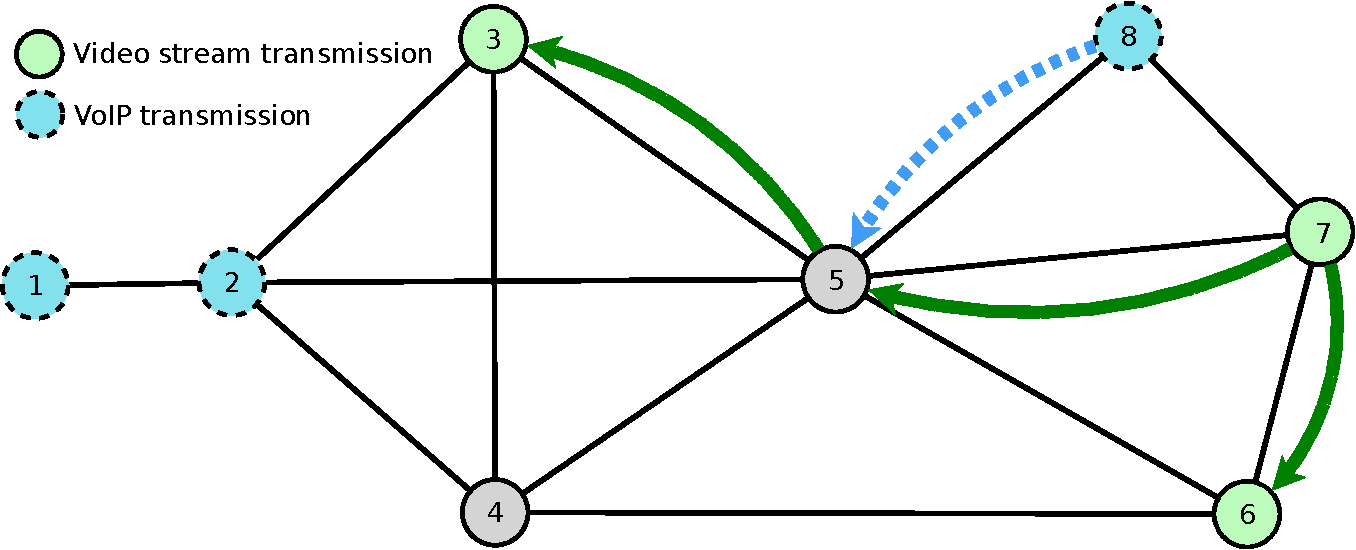
\includegraphics[width=0.9\textwidth]{figures/MulticastCommunicationOne.pdf}
		\caption{Example of an arising transmission problem}
		\label{fig:multicast}
	\end{figure}
	Node $7$ transmits a video stream at time $t$ to the Nodes $3$ and $6$. At time $t+1$, Node $8$ tries to communicate via \VOIP{} with Nodes $2$ and $1$. The intermediate Node $5$ already forwards the bandwidth-consuming video stream and now has to serve two routes. 
%	Consequently, a solution tis mandatory.%...komisch
	
	\section{The Idea}
	As mentioned in Section \ref{sec:Introduction}, the data types have individual specifications, like e.g. available throughput. Furthermore, every data type has a certain priority. Keeping that in mind, the general objective is to reach the most optimal \QOS{} with respect to the available network resources and the individual performance specifications of the data types. To achieve this, every node in this \MANET{} is, apart from the common routing, equipped with additional \QOS{} information. Figure \ref{fig:QoSDecision} shows the architecture of a node with such a \QOS{} routing extension.\\
	Before a node starts transmitting payload, the network capacities have to be compared to the \QOS{} requirements of the payload. This is achieved with transmission request. This transmission requests can either be received from a participating node of the network (\textit{External Transmission Request}) or from a node itself (\textit{Internal Transmission Request}). Both requests contain the \QOS{} requirements of the data type and the priority. \QOS{} requirements specify delay, loss rate and necessary bandwidth of the payload. 
	\begin{figure}[h]
		\centering
		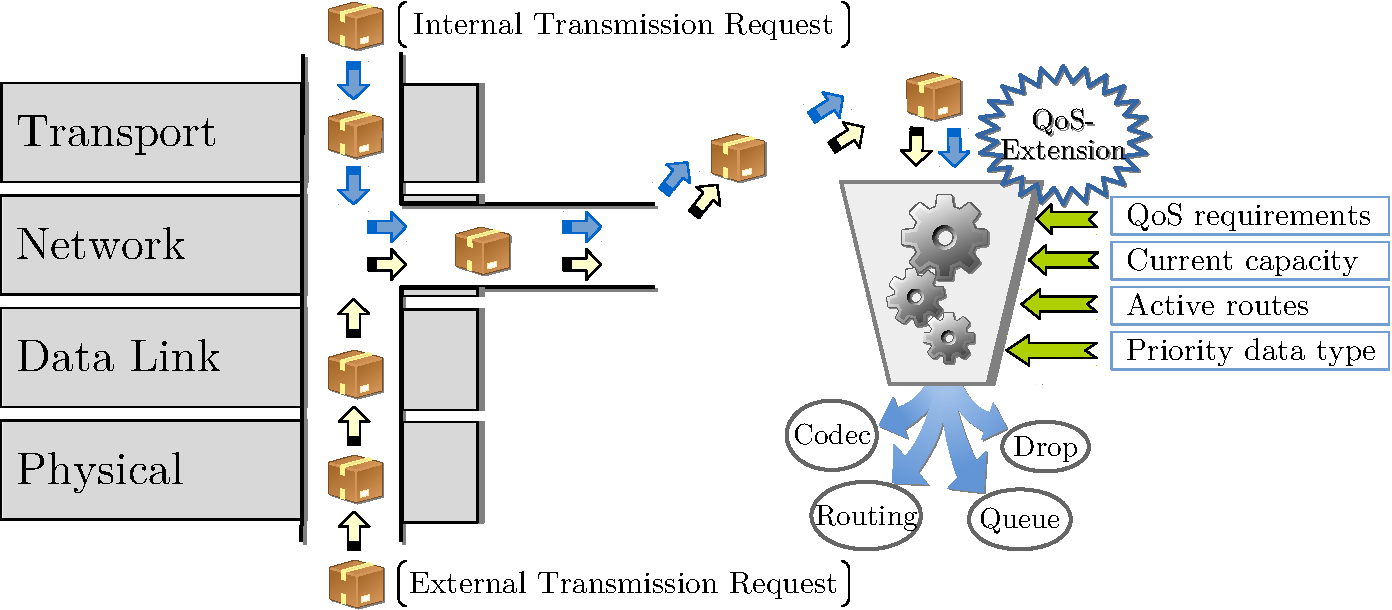
\includegraphics[width=\textwidth]{figures/QoSDecision.pdf}
		\caption{Structure of \QOS{} aware Node in a \MANET{}}
		\label{fig:QoSDecision}
	\end{figure}
	 The \textit{Internal Transmission Request} is triggered from an application running on the radio. Such requests cross the upper layer till they arrive at the \QOS{} extension. There are several factors which influence the treatment of the received request. First, the \QOS{} requirements of the received data type are determined. Then, additional information such as utilization, available bandwidth or active routes of the network has to be examined in order to get an overview of the available resources. Based on this information and depending on the priority of the data type, the request will be treated accordingly. If the node has minimal capacities and low bandwidth because it relays packets of several routes, it might inform the other senders to reduce their sending interval or to drop their packets. If voice has to be transfered under these network conditions, the necessary capacities have to be provided. This can result in the multicast origin having to change the codec of e.g. a video stream to save bandwidth or having to reroute the packets. A picture could be queued and distributed to the multicast receiver when the network load has decreased.\\
	The procedure of an \textit{External Transmission Request} is very similar to the internal transmission request. The node which receives the external request determines the \QOS{} requirements of the received request. Then, factors like available capacity, bandwidth and the number of routes are examined. Again, the node determines the treatment of the request with respect to the priority of the data type, its own possibilities and the \QOS{} requirements of the request. Depending on the results, the request is treated accordingly. If the data type of the request has compared to the other active routes the highest priority and the bandwidth is not sufficient, the origins of resource-consuming routes must be informed to change their transmissions or drop them.\\
	It turns out, that a  management process which affects the network has to be triggered if necessary resources are not available and the \QOS{} requirements can not be met.
	
	\section{Scientific Questions}
	An important characteristic of \MANET{s} is the self organization. This has a fundamental impact on the routing. Basically, routing protocols will determine the fastest route to every multicast receiver with respect to the network load at runtime. Not only time critical requirements, but also data loss rate, throughput, necessary bandwidth and quality have to be taken into account in order to meet the \QOS{}. Accordingly, the following scientific questions have to be investigated:
	\begin{itemize}
		\item How can the current transmissions in the \MANET{} be distributed best in order to fulfill the \QOS{} requirements? 
		\item How can areas with high network utilization be identified?
		\item In case of a sender with higher-priority data determining the best path towards all multicast receivers, how can other senders be informed about changing the behavior of their current transmissions, in order to provide the necessary capacity for the delivery of higher-priority data?
		\item If a multicast route meets the \QOS{} requirements, how can quality be maintained during transmission?
	\end{itemize}

	\section{Related Work}
	In order to create a balanced transmission in the \MANET{} each source has to be able to chose the most suitable route for the requested type of data. To identify possible routes towards the destination, the paper by Helen Bakhsh et al. \cite{RelatedWork:MultiPath} proposes a route discovery algorithm which determines several paths depending on a trust value of each participating node. This value is calculated from the relationship between sent packets and received acknowledgments. For a specified time period the source receives multiple route replies and decides according to the trust value of the route the most suitable path. However, this approach can be used to get an overview of current transmission and the associated data types.\\
	The work of Lu et al. \cite{RelatedWork:QoSWMN} proposes a unicast routing protocol designed for hybrid wireless mesh networks \cite{RelatedWorkContent:WMN}. The algorithm provides a multi-criteria routing functionality with the goal to find either the fastest path or the route with most promising battery level and less link load. The data is divided in urgent and non-urgent. Urgent data is transmitted via the fastest path and non-urgent data uses a route with minimal link load and highest battery level. Simulation results indicate, that the route selection with respect to the data type can effectively reduce the average end-to-end delay when transmitting urgent data. The link load of each node which is part of the received route reply can be extended with GPS coordinates in order to detect areas with high network utilization. The objective is to avoid such areas when searching after a route.\\
	The work of Shams Shafigh et al. manages the network resources of multicast sessions according to the  feedback received by multicast members \cite{ReleatedWork:QoSSessionAdaptation}. The approach tries to adjust the sending rate and the codec of video streams regarding to the received feedback of multicast receivers. The feedback is classified with fuzzy logic \cite{RelatedWorkContent:QoSSessionAdaptationFuzzySets}\cite{RelatedWorkContent:QoSSessionAdaptationFuzzySets2}. The evaluation results show, that with resource adjustment techniques, the packet delivery ratio and the delay can be improved. Adapting the bandwidth is an interesting approach in case of a higher-priority stream requests the capacities. In such a situation the feedback can be used to inform a current transmission about a higher-priority data which could lead to an adjustment of the sending rate.
%	Beforehand, the behavior of a \MANET{} with high network load has to be investigated. The first issue to be analyzed is how the existing multicast routing protocols are coping with the high utilization. 
%	In particular, which result does a network with high utilization produce, where many multicast sessions exist that use \VOIP{}, compared to a network, where a reduced number of multicast sessions exist that stream videos.\\
%	Traditional resource reservation protocols like RSVP are not sufficient for \MANET{s} \cite{MANET:ResourceManagement}
	\section{Early Results}
	Before we try to find a solution for the mentioned research questions, it has to be analyzed which effects occur during transmission in such situations. Especially, if a message is send over multiple nodes and the payload need to be spit. It is expected, that generating a balanced utilization provides better results with respect to delay and loss rate.
	\begin{figure}[h]
		\centering
		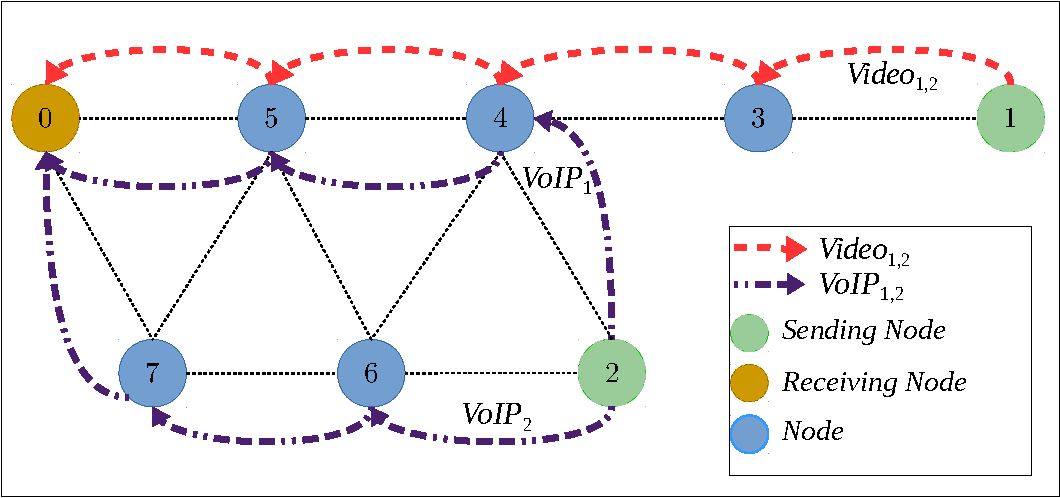
\includegraphics[width=0.8\textwidth]{figures/ScenarioBoth.pdf}
		\caption{Scenario using different routes to destination}
		\label{fig:ScenarioBoth}
	\end{figure}
	%The problem in figure \ref{fig:multicast} could for instance be solved by rerouting the video stream over node $5$. Hence, node $6$ forwards packets towards node $3$ despite receiving the same video stream. Now, node $3$ has free capacities to forward the higher prioritized \VOIP{} stream to node $1$ and $2$.
	To investigate this assumption, we created a scenario, where two different source nodes transmit data to the same destination, shown in Figure \ref{fig:ScenarioBoth}.
	Thereby, the behavior transmitting video and \VOIP{} streams $(Video_1,\VOIP{}_1)$ using the same path is compared with using different routes towards destination $(Video_2,\VOIP{}_2)$.
%	The objective is to analyze the performance with respect to delay and loss rate. Figure \ref{fig:ScenarioBoth} describes the scenario, where this behavior can be analyzed.
	%Node $1$ transmits a video stream to node $0$. To a later time, node $2$ tries to send a \VOIP{} stream to the same destination. The VoIP stream can either be transmitted over the stressed nodes $5$ and $6$ or over $7$ and $8$. Consequently, the path of $VoIP_{1}$ chooses an already stressed path whereas node $2$ routes $VoIP_{2}$ over a path where the intermediate nodes can provide their full bandwidth.
	It is not uncommon that different traffics streams share one path towards the same destination. The routing algorithms AODV \cite{EvaluationAODV} and DSR \cite{Evaluation:DSR} for instance chose the stressed path towards the destination because node $3$ with respect to the introduced scenario would reply with an active route to node $0$. It has to be mentioned, that the data rates of $Video_{1,2}$ provoke a utilized route. With a configured video data rate of $205Kb/s$, the packets of all streams are delivered to the destination. All simulation parameters are shown in Table \ref{tab:ScenarioParameters}.
	\begin{table}
		\centering
		\caption{Configured Simulation parameters}
		\begin{tabular}{l|l} % <-- Alignments: 1st column left, 2nd middle and 3rd right, with vertical lines in between
			\textbf{Type} & \textbf{Value} \\
			\hline
			Simulation time & $65sec$\\
			Bandwidth of  node & $2Mb/s$\\
			Overhead $Video_{1}$ & $227Kb/s$\\
			Overhead $Video_{2}$ & $240Kb/s$\\
			Overhead $VoIP_{1,2}$ & $40Kb/s$
		\end{tabular}
	\label{tab:ScenarioParameters}
	\end{table}\\
	 The plots in Figure \ref{fig:EvaluationResults} illustrate the delivered packets and the delay of the described scenario. Results of the left plot show, that more packets are delivered in total using different paths towards node 0. This becomes clear with a required bandwidth fo $280Kb/s$. There, $Video_1$ delivers $54.994\%$ of the sent packets and the $\VOIP{}_1$ stream loses $5.7737\%$ of the transmitted payload whereas $Video_2$ reaches a delivery rate over $80\%$ and $\VOIP{}_2$ loses $6.8772\%$.
	%Video_1,100,77.805178792,54.993834772
	%VoIP_1,100,100,98.526315789
	%Video_2,100,94.266337855
	%VoIP_2,100,93.719298246
	\begin{figure}[h]
		\pgfplotsset{every axis/.append style={%
				font=\scriptsize,
				ybar,
				xtick=data,
				enlarge x limits=0.5,
				ymajorgrids = true,
				xticklabel={$\pgfmathprintnumber{\tick}$\,Kb/s},
		%		x tick label style={rotate=20},
				ybar=2pt,% configures ‘bar shift’
				bar width=8pt,
		%		nodes near coords,
				point meta=y,
				width=6cm,
		},
				every axis legend/.append style={
					at={(0.5,1.13)},
					anchor=south,
				legend columns=2}
		}%
		
		\centering
		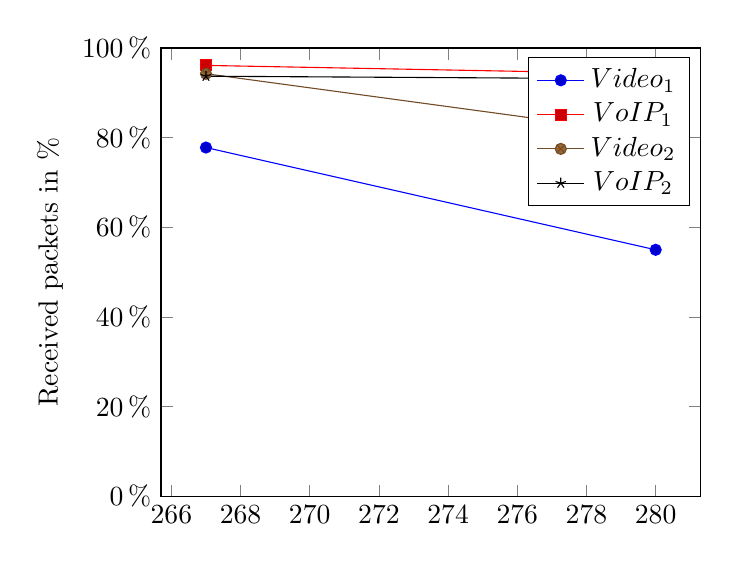
\begin{tikzpicture}
			\begin{axis}
			[
				ymin=0,
				ymax=100,
				yticklabel={$\pgfmathprintnumber{\tick}$\,\%},
				ylabel=
				Received packets in \%
			]
				\addplot coordinates {
					(267,77.805178792)
					(280,54.993834772)
				};
				\addplot coordinates {
					(267,96.126574435)
					(280,94.226315789)
				};
				\addplot coordinates {
					(267,94.266337855)
					(280,80.641183724)
				};
				\addplot coordinates {
					(267,93.719298246)
					(280,93.122807018)
				};
			\legend{$Video_{1}$,$VoIP_{1}$,$Video_{2}$,$VoIP_{2}$}
			\end{axis}
		\end{tikzpicture}
		\hspace{0.2cm}
		%%Video_1,0.018912588134116,0.16371418644307,0.78227163420997
		%%VoIP_1,0.007258126063521,0.015915055324186,0.029224751686324
		%%Video_2,0.016676869124132,0.058117295307285,0.24275129073046
		%%VoIP_2,100,0.00688998462546,0.016873183858963,0.024452734078329
		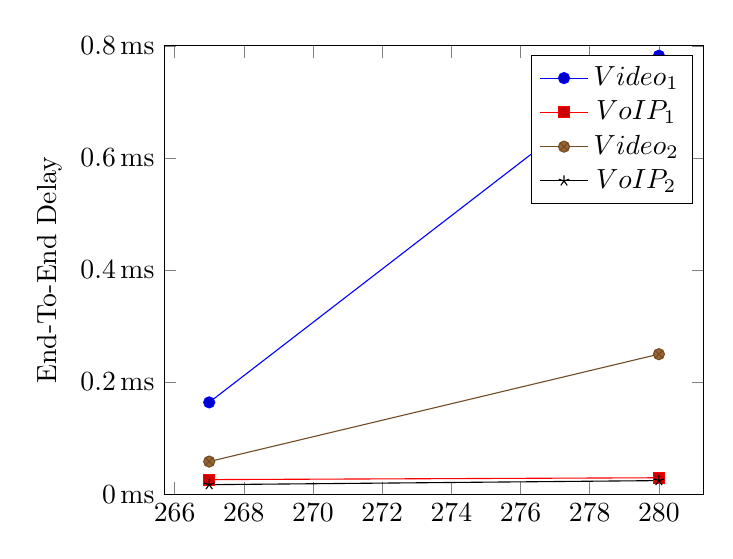
\begin{tikzpicture}
			\begin{axis}
			[
				ymin=0.0,
				ymax=0.8,
				yticklabel={$\pgfmathprintnumber{\tick}$\,ms},
				ylabel=End-To-End Delay
			]
				\addplot coordinates {
				(267,0.16371418644307)
				(280,0.78227163420997)
			};
			\addplot coordinates {
				(267,0.025915055324186)
				(280,0.029224751686324)
			};
			\addplot coordinates {
				(267,0.058117295307285)
				(280,0.24975129073046)
			};
			\addplot coordinates {
				(267,0.016873183858963)
				(280,0.024152734078329)
			};
				\legend{$Video_{1}$,$VoIP_{1}$,$Video_{2}$,$VoIP_{2}$}
			\end{axis}
		\end{tikzpicture}
		\caption{Received packets in percent and associated delay with respect to video and VoIP streams}
		\label{fig:EvaluationResults}
	\end{figure}
	The high loss rate of $Video_{1}$ may be due to an arising congestion. The end to end delay in the left plot reinforce this assumption. Here, $Video_{1}$ produces a noticeable high delay with a required bandwidth of $280Kb/s$. This is because the intermediate nodes do not have enough capacities to forward packets of two routes. In general, using the same path to the destination creates a higher delay and the results show that less packets are lost when using different paths. Based on the results, the next step is to identify nodes with low available bandwidth. The idea is to exclude them when searching after a path in order to provoke a balanced utilization. 
	
%	 This also leads to the question, how  guaranteed to meet the \QOS{} requirements during transmission? 
%	In partially or fully meshed \MANET{s}, several routes from a source to a unicast sink or a  multicast exist. We assume that a malicious node is already present in the network and the fake routes are established as well. How is the behavior of the network with respect to the associated routing during such an attack. Does the blackhole attack have different impact to the packet delivery related to unicast and multicast routing? The topology must provide several routes to sources in order to bypass the malicious node.  path Does a threshold during a blackhole attack exist where one malicious node
%	rotocolls (GKMP)\cite{MANET:GKMPs} in \MANET{s} where a authority exists which is responsible for key management, a Routing Service (RS) exists which is responsible for finding the most efficient route to the requested destination. This component can equal to the \GKMP{s} either be a central instance or a elected, participating node in the \MANET{}. To meet the requirement to find requested routes from an arbitrary host, the \RS{} most be equipped with the knowledge of the actual topology of the network.  The figure .. illustrates the architecture of the 

%	The first aspect to be investigated is: With respect to the number of participating host and the utilization of the \MANET{}, how das the behavior change during the attack.

%	QoS of MANet Through Trust Based AODV Routing Protocol by
%	Exclusion of Black Hole Attack shows a trust model on a unicast manet communication network Trust model between nodes 

%
%
%
% ---- Bibliography ----
%
\begin{thebibliography}{5}
%

\bibitem{SDR}
Harris, F. j.: Software defined radio. In: International Conference on Signals and Electronic Systems (2008) 

\bibitem {military:manet}
Burbank, J. L., Chimento P. F., Haberman, B. K., Kasch W. T.: Key Challenges of Military Tactical Networking and the Elusive Promise of MANET Technology. In: IEEE Communications Magazine (2006)

\bibitem{military:narrowband}
Leduc, J., Antweiler, M., Maseng, T.: Spectrum issues of NATO narrowband waveform: On the spectral efficiency of CPM-Modulation with small modulation indices. In: Military Communications and Information Systems Conference (MCC) (2012)
%\bibitem{MANET:ResourceManagement}
%Ganesh Datey, S., Ansari, T.:Mobile Ad-Hoc Networks Its Advantages and
%Challenges. In: International Journal of Electrical and Electronics Research (A.S.M) (2015)

\bibitem{Video:Bandwidth}
Ozer, J.:Streaming 101: The Basics – Codecs, Bandwidth, Data Rate and Resolution. \url{https://streaminglearningcenter.com/articles/streaming-101-the-basics-codecs-bandwidth-data-rate-and-resolution.html}. Accessed 05 Feb 2009

\bibitem{RelatedWork:MultiPath}
Bakhsh, H., Zhang, N., Carpenter, A.: TADL: A Trust-Aware Dynamic Location-Based Protocol Suite For Discovering Multiple Paths in MANETs. In: Proceedings of the 2015 International Conference on Distributed Computing and Networking (2015)

\bibitem{RelatedWork:QoSWMN}
Lu, L., Jiang, H., Han, G., Ma and Renke Sun, S.: Multi-criteria routing metric for supporting data-differentiated service in hybrid wireless mesh networks in coal mines. In: International Journal of Distributed Sensor Networks (2017)

\bibitem{RelatedWorkContent:WMN}
Akyildiz, Ian F., Wang, X., Wang, W.: Wireless mesh networks: a survey. In: Wireless mesh networks (2005)

\bibitem{ReleatedWork:QoSSessionAdaptation}
Shams Shafigh, A.,Lorenzo Veiga, B., Glisic, S.: Cross layer scheme for quality of service aware multicast routing in mobile ad hoc networks. In: Journal
Wireless Networks (2018)

\bibitem{RelatedWorkContent:QoSSessionAdaptationFuzzySets}
Zadeh, L. A.: Fuzzy sets. In: Information and Control (1965)

\bibitem{RelatedWorkContent:QoSSessionAdaptationFuzzySets2}
Zadeh, A.: Outline of a New Approach to the Analysis of Complex Systems and Decision Processes. In: IEEE Transactions on Systems, Man, and Cybernetics (1973)

\bibitem{EvaluationAODV}
C. E. Perkins and E. M. Royer.: Ad-hoc on-demand distance vector routing. In: Mobile Computing Systems and Applications (1999)
\bibitem{Evaluation:DSR}
B. Johnson, David and Maltz, David.:Dynamic Source Routing in Ad Hoc Wireless Networks. In: Mobile Computing (1999)
%\bibitem{RelatedWork:QoSWMN}
%Sathya, P., Sathiskumar, N.R., Ramasamy, K.: Qos Multicast Routing Algorithm For MANET. In: International Journal Of Engineering And Computer Science (2017)



%\bibitem {mich:tar}
%Michalek, R., Tarantello, G.:
%Subharmonic solutions with prescribed minimal
%period for nonautonomous Hamiltonian systems.
%J. Diff. Eq. 72, 28--55 (1988)
%
%\bibitem {tar}
%Tarantello, G.:
%Subharmonic solutions for Hamiltonian
%systems via a $\bbbz_{p}$ pseudoindex theory.
%Annali di Matematica Pura (to appear)
%
%\bibitem {rab}
%Rabinowitz, P.:
%On subharmonic solutions of a Hamiltonian system.
%Comm. Pure Appl. Math. 33, 609--633 (1980)

\end{thebibliography}

\end{document}
